\chapter{DUNE Detector Overview}
\label{vl:tc-dune_overview}

The \dword{dune} far detector consists of... picture of SP and DP detectors...

\dword{tc} works with consortia through the \dword{tb} to identify and
resolve technical issues.  As defined in the \dword{dune} Management
Plan (DMP), \dword{dune} \dword{tb} generates technical solutions and
recommends technical decisions to the \dword{dune} collaboration
\dword{exb}, which comprises all consortia scientific and technical
leads. The board meets regularly (approximately monthly) to review and
resolve technical issues with detector construction. It reports
through the \dword{exb} to collaboration management. The \dword{dune}
\dword{tb} is chaired by the \dword{dune} \dword{tcoord}. The
\dword{tc} engineering team meets regularly (approximately weekly) to
discuss detailed technical issues.  \Dword{tc} is not responsible for
financial issues, which are referred to the \dword{exb} and
\dword{rcoord}.

\Dword{tc} has several major project support tasks:
\begin{itemize}
\item Ensure that each consortium has a well defined and complete
  scope, that interactions between the consortia are sufficiently well
  defined, and that any remaining scope is covered by \dword{tc}
  through \dword{comfund} or flagged as missing scope to the
  \dword{exb} and \dword{rcoord}. In other words, ensure that the full
  detector scope is identified. Monitor interactions and consortia
  progress in delivering their scope.
\item Develop an overall project \dlong{ims}
  that includes reasonable production schedules, testing plans and a
  well developed installation schedule from each consortium. Monitor
  the \dword{ims} as well as individual consortium schedules.
\item Ensure that appropriate engineering and safety standards are
  developed, understood and agreed to by all key stakeholders and that these
  standards are conveyed to and understood by each
  consortium. Monitor the design and engineering work.
\item Ensure that all \dword{dune} requirements on \dword{lbnf} for
  conventional facilities, cryostat and cryogenics are clearly
  defined and understood by each consortium. Negotiate scope
  boundaries with \dword{lbnf}. Monitor \dword{lbnf} progress on
  final conventional facility, cryostat and cryogenics
  design and implementation.
\item Ensure that technical issues associated with scaling from
  \dword{protodune} have sufficient resources to enable the detector to be fully integrated and
  installed (converging on
  decisions made by the consortia).
\item Ensure that each consortium has fully developed and reviewed
  integration plans, \dword{qc} processes, requirements for
  the \dword{itf} and installation plans..
\end{itemize}

\Dword{tc} is responsible for technical quality and the schedule but
not for consortia funding or budgets.  \Dword{tc} will try to resolve
any issues it can but will likely push all financial issues to the
\dword{tb}, \dword{exb} and \dword{rcoord} for resolution.

\Dword{tc} maintains a web
page\footnote{\url{https://web.fnal.gov/collaboration/DUNE/DUNE\%20Project/\_layouts/15/start.aspx\#/}.}
with links to project documents. \Dword{tc} also maintains
repositories of project documents and drawings. These include the
\dword{wbs}, schedule, risk register, requirements, milestones,
strategy, detector models and drawings that define the \dword{dune}
detector.

\section{\dword{dune} Project Description}

The following sections describe the systems that track the progress of
the \dword{dune} project as well as the ways in which this large,
distributed organization is managed.

The \dword{dune} project builds on significant development in previous
large \dword{lartpc} detectors (ICARUS and MicroBooNE) and on
substantial development from LBNE and LBNO. One of the most important
elements that has significantly advanced the project development is
the successfully construction and operation of the \dword{protodune}
detectors. These detectors use full-size \dword{dune} components and
processes. The construction of \dword{protodune} has established
teams, production lines, QA and QC processes, installation, operation
and performance of the final \dword{dune} detectors. Based on the
success of \dword{protodune}, \dword{dune} has reached advanced technical
maturity, approaching (80\%). The designs have significantly advanced
from \dword{protodune} to \dword{dune}. Most subsystems completed
\dword{pdr} or 60\% reviews on design modifications beyond
\dword{protodune} in advance of the \dword{tdr}. The overall level of
design maturity is now $\sim$90\%. The breakdown of the design maturity
level for \dword{dsp} by subsystem is provided in
Table~\ref{tab:designmaturity}. The table shows the final \dword{dune}
design maturity at the time of \dword{protodune} and now at the time
of the \dword{tdr}, along with the estimated design effort or weight
of each subsystem. The \dword{apa} conceptual design was developed in
2010 and prototyped at 40\% scale and again in the 35-ton detector. The version
deployed in \dword{pdsp} is close to that for \dword{dsp} (85\%). The
cold electronics low noise system design, including feedthroughs,
cables and grounding, was successfully prototyped at large scale in
MicroBooNE and \dword{pdsp} and is 90\% mature. The front end chip has
gone through eight iterations and was successfully demonstrated in
MicroBooNE and \dword{pdsp} (90\%). The frontend motherboard has gone
through a similar number of iterations and was successfully
demonstrated in \dword{pdsp} (80\%). The ADC chip has evolved from a
previous version used in CMOS 180~nm technology that was tested to $-50\circ$C. (50\%). Key
elements of the COLDATA chip have been prototyped (25\%). The HV
design has evolved from ICARUS, MicroBooNE and the 35-ton detector.  It
has been prototyped in subsequent runs of the 35-ton detector and
demonstrated in \dword{pdsp} (80\%). The photon system ARAPUCA design
has been prototyped at small scale and in \dword{pdsp} (20\%). The
mechanical design has been extensively developed using the 35-ton
detector and \dword{pdsp} (85\%). The DAQ artdaq backend has been
developed in several experiments, including the 35-ton detector and
\dword{pdsp}. The DAQ FELIX frontend has been developed by ATLAS and
prototyped in \dword{pdsp}.
\begin{dunetable}
  [\dword{dsp} design maturity]
  {|p{0.1\linewidth}|rp{0.1\linewidth}|rp{0.25\linewidth}|rp{0.2\linewidth}|}
  {tab:designmaturity}
  {\dword{dsp} design maturity}
  System & Weight & \dword{protodune} & \dword{dune}   \\ \toprowrule
  DSS & 10\% & 75\% &  85\% \\ \colhline
  APA & 30\% & 85\% &  95\% \\ \colhline
  CE  & 20\% & 80\% &  90\% \\ \colhline
  PDS & 10\% & 50\% &  65\% \\ \colhline
  HVS & 15\% & 80\% &  95\% \\ \colhline
  DAQ & 10\% & 60\% &  80\% \\ \colhline
  CISC & 5\% & 80\% &  90\% \\ \colhline \colhline
  Total& 100\% & 76\% & 90\% \\ \colhline
\end{dunetable}

The design maturity of the \dword{ddp} detector is also quite
advanced. It builds on working noble liquid \dwords{tpc} for dark
matter and neutrinoless double beta decay experiments. A significant
benchmark is the operation of the $3\times1\times1$ demonstrator at
CERN. A critical test will be the operation of \dword{pddp} at CERN. A
similar table of design maturity for \dword{ddp} will be included
here.

%%%%%%%%%%%%%%%%%%%%%%%%%%%%%%%%
\section{Work Breakdown Structure (WBS)}
\label{sec:fdsp-coord-wbs}

The \dword{dune} \dword{wbs} has six categories at level 1 as shown in
Table~\ref{fig:WBS_level2}.  
\begin{dunefigure}[\dword{dune} \dword{wbs} at level 2]{fig:WBS_level2}
  {High level \dword{dune} \dword{wbs} to level 2.}
  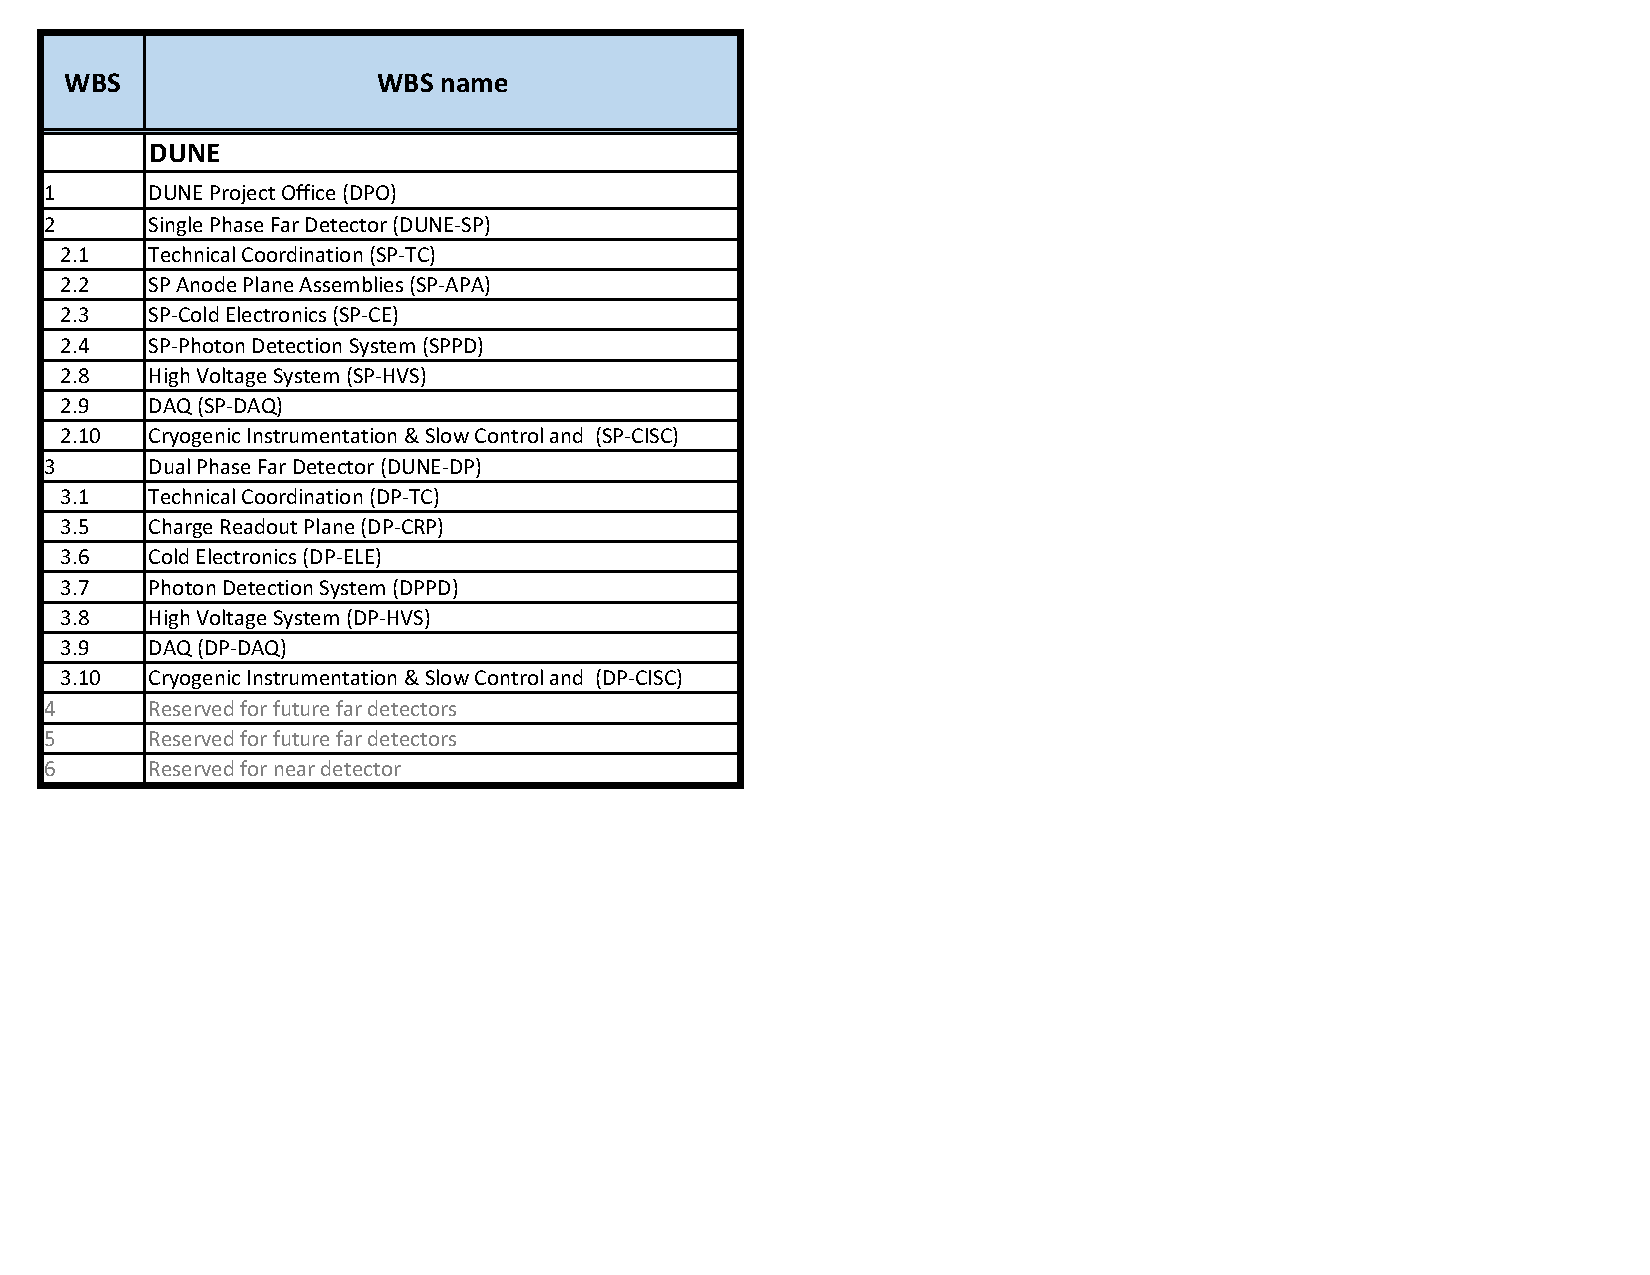
\includegraphics[width=0.75\textwidth]{WBS_level2}
\end{dunefigure}
At level 2, the \dword{wbs} breaks down into seven items, both
for single-phase and dual-phase far detectors, including the \dword{tc}
functions associated with installation.

Each subsystem \dword{wbs} is owned by the associated consortium. The
consortia \dword{wbs} follow a common format with the first level
(level 3) broken down in rough time sequence into the following
categories:
\begin{enumerate}
  \item Management
  \item Physics and Simulation
  \item Design, Engineering and R\&D
  \item Production Setup
  \item Production
  \item Integration (ITF)
  \item Installation (\surf)
\end{enumerate}
Subsequent levels in the \dword{wbs} generally follow consortia subsystem structure.
This \dword{wbs} has been used as the framework to capture the costs
for the overall \dword{dune} project cost estimate.
